\section{Separación de responsabilidades}

La primera decisión del desarrollo fue evitar que la operación aritmética quedara mezclada con los detalles propios de la placa. La \tech{ALU} solo necesita recibir dos operandos y un código de operación; no debería conocer de dónde provienen esos datos ni cómo se presentan al usuario. Los switches, pulsadores, registros y LED pertenecen a otra responsabilidad.

Con ese criterio, el diseño quedó dividido en tres bloques. \texttt{alu} implementa el cálculo combinacional; \texttt{button\_input} incorpora las entradas manuales al dominio del reloj; y \texttt{alu\_top} conserva los valores ingresados y conecta el conjunto con la \tech{Basys 3}. Esta separación permite verificar cada problema de manera aislada antes de probar la integración.

La figura~\ref{fig:arquitectura-conceptual} resume el recorrido completo. Los ocho switches forman un bus compartido: el usuario prepara un valor y el pulsador correspondiente decide en qué registro debe guardarse. Una vez almacenados A, B y el opcode, la ALU actualiza de manera combinacional el resultado y los indicadores.

\begin{figure}[H]
	\centering
	\begin{tikzpicture}[
		node distance=1.55cm and 1.55cm,
		block/.style={draw=coderule, fill=codeback, rounded corners=2mm,
			minimum height=1.15cm, align=center, thick, inner xsep=6pt},
		io/.style={block, draw=codeviolet},
		flow/.style={-{Latex[length=2.4mm]}, thick, draw=codeviolet},
		control/.style={-{Latex[length=2.2mm]}, thick, dashed, draw=codeblue},
		signal/.style={font=\small, fill=white, inner sep=2pt}
	]
		\node[io, text width=2.15cm] (switches) {Switches\\\texttt{SW7--SW0}};
		\node[block, text width=3.05cm, right=of switches] (registers)
			{Registros\\A, B y opcode};
		\node[block, text width=2.05cm, right=of registers] (alu)
			{Núcleo\\\texttt{alu}};
		\node[io, text width=2.35cm, right=of alu] (leds)
			{LED\\resultado y Z/C/V};

		\node[io, text width=2.15cm, below=of switches] (buttons)
			{Pulsadores\\carga y reset};
		\node[block, text width=3.05cm, right=of buttons] (sync)
			{Sincronizadores\\\texttt{button\_input}};

		\draw[flow] (switches) -- node[signal, above=2pt] {bus} (registers);
		\draw[flow] (registers) -- (alu);
		\draw[flow] (alu) -- (leds);
		\draw[control] (buttons) -- (sync);
		\draw[control] (sync.north) --
			node[signal, right=4pt] {habilitación} (registers.south);

		% El contorno identifica el dominio síncrono sin convertir el dibujo
		% conceptual en un esquema de cada conexión de reloj.
		\node[draw=codeblue, dashed, rounded corners=2mm,
			fit=(registers)(sync), inner sep=7pt] (clockdomain) {};
		\node[signal, text=codeblue, anchor=north east]
			at ([yshift=-2pt]clockdomain.south east)
			{dominio de reloj: \SI{100}{\mega\hertz}};
	\end{tikzpicture}
	\caption{Arquitectura conceptual y flujo de datos del sistema.}
	\label{fig:arquitectura-conceptual}
\end{figure}

\section{Flujo de operación}

El ingreso se realiza en tres pasos. Primero se configura A en los switches y se pulsa el botón izquierdo. Luego se repite el procedimiento para B con el botón derecho. Por último se colocan los seis bits del opcode y se utiliza el botón superior. Los pulsadores no escriben directamente en la ALU: atraviesan los sincronizadores y habilitan registros que conservan cada valor.

Esta diferencia es importante. Los operandos pueden cargarse en momentos distintos porque los registros mantienen su contenido entre pulsaciones. Cuando el último valor cambia, la lógica combinacional recalcula inmediatamente la salida. El usuario no necesita una orden adicional de ejecución: cargar el opcode completa la entrada y los LED reflejan el resultado.

\begin{table}[H]
\centering
\begin{tabularx}{\textwidth}{L{3.2cm}L{3.5cm}Y}
\toprule
\textbf{Etapa} & \textbf{Módulo responsable} & \textbf{Descripción} \\
\midrule
Ingreso manual & Recursos de la Basys 3 & Los switches presentan un valor y los pulsadores eligen su destino. \\
Sincronización & \texttt{button\_input} & Cada pulsador atraviesa dos flip-flops antes de utilizarse como control. \\
Almacenamiento & \texttt{alu\_top} & Tres registros conservan A, B y opcode; el reset tiene prioridad. \\
Cálculo & \texttt{alu} & La lógica combinacional selecciona una de ocho operaciones y genera Z/C/V. \\
Presentación & \texttt{alu\_top} & Los ocho bits de resultado y los tres indicadores se conectan a LED. \\
\bottomrule
\end{tabularx}
\caption{Flujo funcional desde los controles hasta la salida.}
\end{table}

% La tabla de decisiones necesita una página casi completa. El salto evita
% separar el título y su introducción de la evidencia que presentan.
\clearpage
\section{Decisiones de diseño}

Las decisiones de la tabla~\ref{tab:decisiones} establecen tanto el comportamiento del circuito como las condiciones bajo las cuales debe utilizarse. Reunirlas en un solo lugar evita que una elección importante quede oculta dentro de un fragmento de código.

\begin{table}[H]
\centering
\small
\begin{tabularx}{\textwidth}{L{3.8cm}L{5.0cm}Y}
\toprule
\textbf{Decisión} & \textbf{Motivo} & \textbf{Consecuencia} \\
\midrule
Separar \texttt{alu} de \texttt{alu\_top} & Aislar el cálculo de la interfaz física. & El núcleo puede verificarse sin reloj ni controles de placa. \\
Compartir los ocho switches & Reutilizar una interfaz limitada para tres entradas. & A, B y opcode deben cargarse de forma secuencial. \\
Sincronizar cada pulsador con dos flip-flops & Reducir el riesgo de propagar metastabilidad. & La habilitación aparece varios ciclos después de la acción manual. \\
Usar cargas activas por nivel & Mantener una lógica de control simple. & Una pulsación sostenida recarga el mismo valor; no se genera un pulso único. \\
No implementar antirrebote & Las recargas son inocuas si el bus permanece estable. & Los switches no deben modificarse hasta que el botón se haya liberado. \\
Definir cero para opcodes inválidos & Cubrir todas las combinaciones y evitar memoria implícita. & El indicador Z se activa ante un código no reconocido. \\
Reservar carry para ADD & Mantener una semántica inequívoca del indicador. & SUB no informa préstamo; C permanece en cero. \\
Dar prioridad al reset & Asegurar un estado conocido incluso si hay cargas activas. & A, B y opcode se borran mientras el reset sincronizado esté activo. \\
Exceptuar switches y LED del timing & Modelar que no poseen una relación temporal externa definida. & El reporte temporal no demuestra la estabilidad manual del bus ni el retardo hacia los LED. \\
\bottomrule
\end{tabularx}
\caption{Decisiones de diseño, fundamentos e implicancias.}
\label{tab:decisiones}
\end{table}

\clearpage
\section{Organización del proyecto}

La organización de las fuentes reproduce la arquitectura. Cada módulo de diseño posee un banco de pruebas dedicado y las restricciones físicas permanecen separadas del código RTL.

\begin{table}[H]
\centering
\begin{tabularx}{\textwidth}{L{5.4cm}Y}
\toprule
\textbf{Archivo} & \textbf{Función} \\
\midrule
\texttt{alu.sv} & Operaciones e indicadores de la ALU. \\
\texttt{button\_input.sv} & Sincronización de un pulsador. \\
\texttt{alu\_top.sv} & Registros e integración con la placa. \\
\texttt{alu\_tb.sv} & Verificación del núcleo combinacional. \\
\texttt{button\_input\_tb.sv} & Verificación del sincronizador. \\
\texttt{alu\_top\_tb.sv} & Verificación de cargas, reset e integración. \\
\texttt{basys3.xdc} & Pines y restricciones temporales. \\
\texttt{scripts/}\newline\texttt{create\_sync\_project.tcl} & Creación reproducible del proyecto de Vivado. \\
\bottomrule
\end{tabularx}
\caption{Archivos principales del trabajo práctico.}
\end{table}

La jerarquía mostrada por \tech{Vivado} en la figura~\ref{fig:sources} confirma esa división. Bajo \texttt{alu\_top} aparecen cuatro instancias de \texttt{button\_input}, una por pulsador, y la instancia \texttt{alu\_core}. Los testbenches se encuentran en \textit{Simulation Sources} y no forman parte del circuito sintetizado.

\begin{figure}[H]
	\centering
	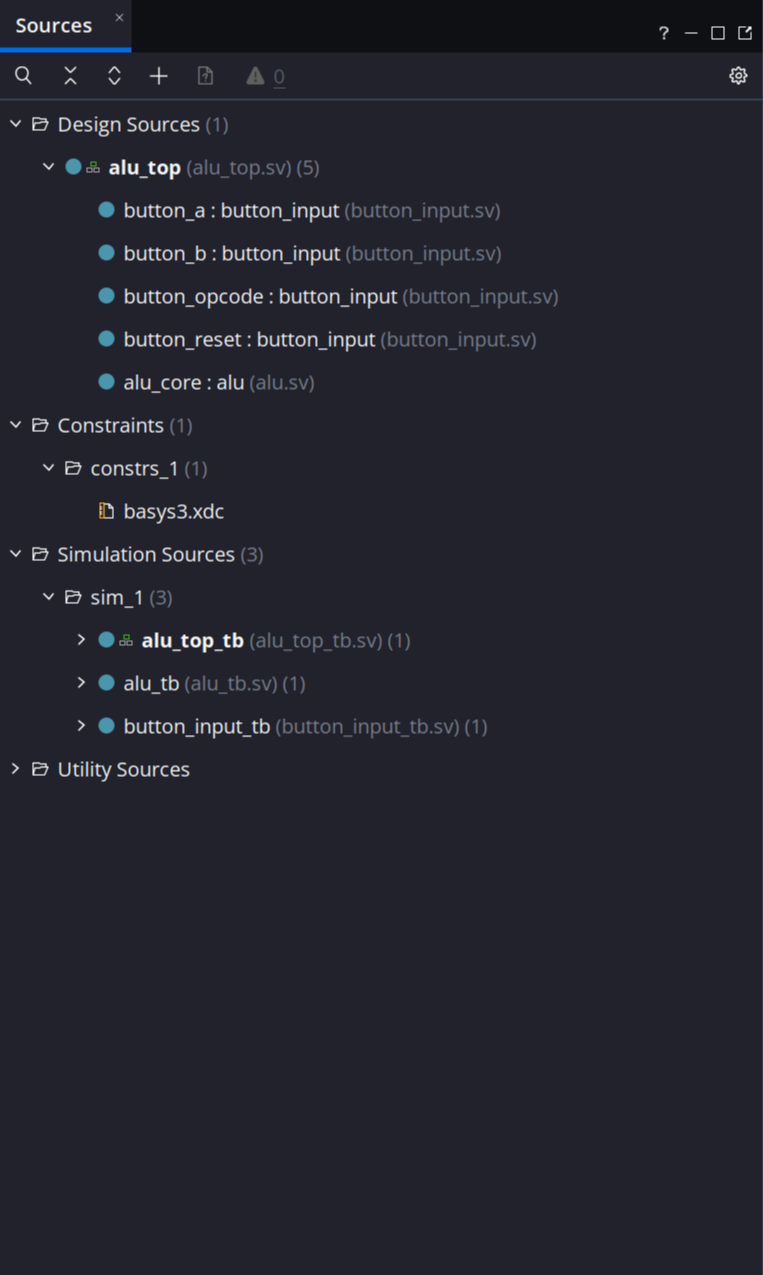
\includegraphics[height=0.66\textheight]{img/sources.png}
	\caption{Jerarquía de módulos, restricciones y fuentes de simulación.}
	\label{fig:sources}
\end{figure}
